\documentclass[IJPHM, 2026, 0]{phmsociety}
\renewcommand{\paperNumber}{0}
\usepackage{fontspec}
\setmainfont{Times New Roman}
\usepackage{amsmath,amssymb,graphicx,booktabs,tabularx,array,etoolbox}
\usepackage{xurl}
\usepackage{microtype}
\providecommand{\tightlist}{\setlength{\itemsep}{0pt}\setlength{\parskip}{0pt}}
\setcounter{secnumdepth}{3}
\setlength{\emergencystretch}{3em}
\fancyhead{}
\fancyhead[L]{\footnotesize\textsc{International Journal of Prognostics and Health Management}}
\fancyhead[R]{\footnotesize\textsc{Mozafari}}
\fancypagestyle{plain}{%
  \fancyhead{}%
  \fancyfoot{}%
  \fancyfoot[L]{\footnotesize International Journal of Prognostics and Health Management, ISSN2153-2648, \publicationYear~\paperNumber}%
  \fancyfoot[R]{\small\thepage}%
}
% Single-author form of the supplied licence macro; the class itself is unchanged.
\patchcmd{\phmLicenseFootnote}{~et al.}{.}{}{\errmessage{Licence macro patch failed}}
\AtBeginDocument{\special{pdf:docinfo << /Author (Amirhossein Mozafari) >>}}
\begin{document}
\title{Compatibility of Quantile and Event-Probability Outputs in Remaining Useful Life Prediction: Event-Head Corruption Detection and Scoring Changes under Label-Free Projection}
\author{Amirhossein Mozafari\authorNumber{1}}
\address{\affiliation{1}{Department of Computer Science, Sharif University of Technology, Tehran, Iran}{\email{amir.mozafari04@sharif.edu}}}
\maketitle
\pagestyle{fancy}
\thispagestyle{plain}
\phmLicenseFootnote{Amirhossein Mozafari}
\begin{abstract}%
Multi-head models for remaining useful life (RUL) prediction can report quantiles and near-term failure probabilities that disagree, complicating maintenance interpretation. We study a quantile-implied incompatibility distance \(d\) and a label-free projection, \(p_{\mathrm{proj}}=\operatorname{clip}(p,L,U)\). On C-MAPSS, the original eight groups share 707 test engines. Flags detect gross uniform event-head replacement and probability inversion, whereas a -1 logit shift lowers their rate. Flags concentrate near the event threshold: 49.7\% within RUL 20--40 versus 8.2\% elsewhere. RUL-only Brier associations are positive overall but differ in sign after probability-and-band adjustment. The pooled point-error association is undetected; its approximate 80\%-power minimum detectable effect is 162 cycles squared. Across the expanded 44 groups, projection slightly lowers pooled Brier and NLL, with inconsistent group effects. Its Brier gain is resolved in FD002 and FD004 and unresolved in FD001 and FD003. TrainOff has lower pooled Brier and NLL than projection alone, largely driven by FD002, but has worse Brier than projection in 17 groups, including all 11 FD001 groups, and worse NLL in 15 by point estimate. No paired CI compares these paths. The exploratory study uses examined data from a single benchmark; projection guarantees the necessary structural bounds, while its scoring benefit remains empirical and varies across groups.
\end{abstract}
\textbf{Keywords:} remaining useful life; C-MAPSS; quantile--probability compatibility; calibration; label-free projection.

\section{Introduction}

Maintenance interpretation depends on what a prognostic output describes. Conditional RUL quantiles summarize the predicted distribution of time to failure, whereas an event head estimates the probability of failure within a specified horizon. A model that supplies both outputs should present a consistent account of the same event. A low near-term failure probability alongside quantiles that place failure before the horizon, or the converse disagreement, can make the outputs difficult to reconcile when considering maintenance actions. This study examines that structural disagreement; it does not evaluate maintenance decisions or safety outcomes.

Multi-head RUL models can estimate quantiles and event probabilities separately, without requiring them to correspond to one conditional distribution. Weighted classification losses can further displace the event probability from the unweighted target. We examine this compatibility problem on C-MAPSS \cite{saxena2008cmapss, saxena2008damage}. Quantile ordering supplies necessary bounds on the event probability \cite{koenker1978regression}, allowing disagreement to be identified without observing the outcome.

Structural compatibility, probability calibration and prediction error answer different questions. An output can satisfy the quantile-implied bounds and still be inaccurate or poorly calibrated. Conversely, a probability transformation can improve a proper score while increasing disagreement with the quantiles. The practical question is therefore whether the diagnostic identifies useful forms of disagreement and what scoring trade-offs arise when that disagreement is removed.

The study makes the following contributions:

\begin{itemize}
\tightlist
\item
  Formalizes a label-free compatibility diagnostic from quantile ordering and evaluates projection onto its necessary probability bounds.
\item
  Tests sensitivity to event-head corruption and quantile perturbation, and examines threshold concentration, error associations and detectable effects on C-MAPSS.
\item
  Compares projection with analytical training-weight correction (TrainOff) and fitted post-hoc calibrators across \mbox{44} model groups, reporting both favorable and unfavorable effects.
\end{itemize}

\section{Related work}

Probabilistic forecast assessment separates agreement with observations from concentration of the predictive distribution. Gneiting, Balabdaoui and Raftery distinguish calibration from sharpness \cite{gneiting2007calibrationsharpness}. Gneiting and Ranjan develop prediction spaces for forecast combination and distinguish coherence, probabilistic and conditional calibration, and dispersion \cite{gneiting2013combining}. These distinctions motivate assessing structural compatibility separately from outcome-based calibration. They do not establish the usefulness of the present flag or supply its finite-grid cross-head construction.

Quantile ordering provides the basis for the construction. Koenker and Bassett introduce regression quantiles for estimating conditional quantile functions \cite{koenker1978regression}. Chernozhukov, Fernández-Val and Galichon study monotone rearrangement to remove crossings in estimated quantile and probability curves \cite{chernozhukov2010crossing}. Ordering the quantiles addresses crossings within those estimates, but does not by itself make a separate event head agree with them. The bounds studied here express that additional requirement.

Proper scores assess predictions against realized outcomes. Gneiting and Raftery develop the proper-scoring framework used for our Brier and NLL comparisons \cite{gneiting2007scoring}. Guo et al.~examine post-hoc neural-network calibration and temperature scaling \cite{guo2017calibration}, while Silva Filho et al.~review calibration definitions, metrics and post-hoc maps \cite{silvafilho2023calibration}. These works support comparing projection with probability calibration, without implying a particular empirical ranking on the engines studied here.

For RUL prediction, Javanmardi and Hüllermeier conformalize point predictors into intervals and evaluate them on C-MAPSS \cite{javanmardi2023conformal}. Their work addresses interval prediction and coverage. Our question concerns whether quantile and event-probability heads can describe the same event, even before their predictions are compared with outcomes. Compatibility is a necessary structural condition rather than an interval-coverage or calibration guarantee.

\section{Methodology: compatibility diagnostic and post-hoc corrections}

\subsection{Quantile-implied probability bounds}\label{quantile-implied-probability-bounds}

Let \(p\) denote the predicted probability of failure within horizon \(h\). For \(h=30\) and quantile levels \(\tau\in\{0.05,0.50,0.95\}\), the ordered quantiles imply the bounds

\begin{equation}
\begin{aligned}
L(h)&=\max\bigl(\{0\}\cup\{\tau:q_\tau\le h\}\bigr),\\
U(h)&=\min\bigl(\{1\}\cup\{\tau:q_\tau>h\}\bigr).
\end{aligned}
\end{equation}

\begin{equation}
d=\max\{L(h)-p,\ p-U(h),\ 0\}.
\end{equation}

The lower bound collects quantile levels whose predicted RUL is at or below the horizon; the upper bound collects levels whose predicted RUL is above it. The distance measures how far the event probability lies outside that interval. Satisfying these inequalities does not establish a calibrated or accurate common distribution. Disagreement can arise from separate estimation, objective weighting, approximation, optimization or sampling effects.

The primary validation flag is \(d>0\). Table \mbox{2} uses the earlier \(d>10^{-6}\) convention. Distances are averaged over all engines, including those with zero distance.

\subsection{Label-free projection}\label{label-free-projection}

Projection replaces the event probability with the closest value within the quantile-implied interval, leaving the quantiles unchanged:

\begin{equation}
p_{\mathrm{proj}}=\operatorname{clip}(p,L,U).
\end{equation}

This operation requires no outcome labels and enforces the necessary bounds by construction. Whether the replacement improves a proper score depends on the observed outcomes and is evaluated separately. Each calibrator can also be followed by the same projection.

\subsection{Weight correction and fitted calibration paths}\label{weight-correction-and-fitted-calibration-paths}

Let \(r\) be the event-head logit, \(\sigma\) the sigmoid function and \(w\) the positive-class weight used in training. The positive-class-weighted BCE population optimum differs from the target event probability. TrainOff removes the corresponding logit offset using the actual training weight; it is an analytical correction, not a map fitted to calibration labels. With temperature \(T\), the three paths are

\begin{equation}
\begin{aligned}
p_{\mathrm{TrainOff}}&=\sigma(r-\log w),\\
p_{\mathrm{Temp}}&=\sigma(r/T),\\
p_{\mathrm{TrainOff+Temp}}&=\sigma((r-\log w)/T).
\end{aligned}
\end{equation}

Temperature is fitted on calibration engines by minimizing binary NLL within the original implementation bounds. Platt calibration fits an affine transformation of the raw logit, \(p_{\mathrm{Platt}}=\sigma(a r+c)\). Isotonic calibration fits a nondecreasing map of the raw probability. Beta calibration uses \(p_{\mathrm{Beta}}=\sigma(c+a\log p-b\log(1-p))\), with the implementation's probability clipping and unconstrained fitted coefficients. Platt and Beta use the implementation's coefficient penalty, excluding the intercept. When calibration outcomes contain only one class, fitted calibration paths use the implementation's smoothed constant probability.

\section{Experimental setup}

\subsection{Benchmark, model groups and evaluation roles}\label{benchmark-model-groups-and-evaluation-roles}

The benchmark models have ordered quantile heads and a separate event head. For the original eight equal-search groups, C-MAPSS fitting/validation/calibration engine counts are \mbox{60}/\mbox{20}/\mbox{20} for FD001 and FD003, \mbox{156}/\mbox{52}/\mbox{52} for FD002, and \mbox{149}/\mbox{50}/\mbox{50} for FD004. Official testing uses each engine's final observed window. LSTM and hybrid each use five seeds fixed before this analysis; the hybrid combines recurrent and causal convolutional branches. Model selection used validation error. Architecture details are provided in the supplement.

The expanded comparison uses existing calibration and test predictions for \mbox{44} groups and \mbox{220} fixed fits on the same \mbox{707} distinct official-test engines. It includes the original eight equal-search groups, the TCN/GRU equal-search extension, the original hybrid runs with their own calibration partitions, and extra LSTM/hybrid/GRU/TCN controls, including the additional LSTM/hybrid CV controls. The expanded roster has \mbox{518} distinct calibration engines across its recorded partitions, compared with \mbox{142} for the original eight groups. Each map is fitted separately on the calibration engines belonging to that fit. The paths are raw, projection, TrainOff, Temp, TrainOff+Temp, Platt, Isotonic and Beta, with each calibration path also followed by projection.

The point target is RUL capped at \mbox{125}, and the event label is true RUL at most 30. Benchmark RMSE and MAE use projected medians in {[}\mbox{0},\mbox{125}{]}. The error-association analysis uses squared error of the original unprojected median. Probability error is the binary quadratic contribution \((p-y)^2\), consistent with proper-scoring assessment \cite{gneiting2007scoring}. Seed variation in the benchmark tables is reported as sample SD.

The main evidence comes from C-MAPSS models held fixed during analysis. Quantile perturbations, weighting comparisons and event-head controls examine different sources of disagreement. The synthetic experiment is a pipeline check with a known data-generating law (Supplement S0a), with its full percentile table in Table S11. It does not validate or benchmark the real-data incompatibility rates.

\subsection{Outcomes, uncertainty and reporting}\label{outcomes-uncertainty-and-reporting}

Engine-level cluster bootstrap intervals keep each engine's complete set of model predictions together. Within each subset, LSTM and hybrid share the same engines, and all five seeds reuse that fleet; the original eight groups are not independent. That roster contains \mbox{707} distinct test-engine clusters and \mbox{142} distinct calibration engines. The expanded \mbox{44}-group roster uses the same \mbox{707} test engines and \mbox{518} distinct calibration engines across its recorded partitions. Calibration partitions differ across fits. Original pooled estimates average architectures within each subset and weight subsets by engine count. Expanded-roster estimates average fixed groups within each engine before weighting subsets by engine count. Pooled adjusted coefficients are weighted averages of group-specific coefficients, rather than a common-slope regression coefficient.

RUL-adjusted regressions use the original cubic capped-RUL covariate and seed intercepts. Additional adjustment includes raw probability and the threshold band. Minimum detectable effects use the approximation specified in Table \mbox{1}; they do not replace an exact power simulation.

NLL uses scoring-time clipping at \(10^{-15}\). ECE5 uses five probability-quantile bins, and ECE10 uses ten equal-width bins. Boundaries use no labels and remain fixed during bootstrap. ECE is averaged across fixed models rather than calculated from a mixture probability.

Rates and their CIs are reported as percentages to one decimal; rate differences are percentage points. Regression coefficients and CIs use three significant figures. Benchmark Brier values retain source precision. Continuous scores, differences and CIs in the controls/projection analysis use three significant figures, with full precision in the companion CSVs. The supplement identifies source files and supplies full-precision companions.

\subsection{Analysis development and exploratory scope}\label{analysis-development-and-exploratory-scope}

The original prespecified joint rule returned ``not informative'' (Supplement S0). After examining benchmark and diagnostic results in the original eight groups, we added the error-association follow-ups, positive controls, detectable-effect assessment and direct projection, then expanded the comparison to \mbox{44} model groups and additional calibrators. Later protocols specified each calculation before it was run, but the questions were chosen after earlier results. The expansion tests consistency across model configurations on the same test engines; it is not validation on an independent dataset. Supplement S0d documents the full analysis sequence.

\section{Results and discussion}

\subsection{Baseline incompatibility and perturbation robustness}\label{baseline-incompatibility-and-perturbation-robustness}

Table \mbox{2} summarizes incompatibility frequency and distance in the original eight equal-search groups. Each group averages five fits on the same test engines. These rates describe disagreement between outputs, not the probability that a model is faulty.

\begin{table*}[t]
\centering
\normalsize
\setlength{\tabcolsep}{3pt}
\renewcommand{\arraystretch}{1.12}
\setcounter{table}{1}
\caption{Frozen C-MAPSS compatibility results, mean ± sample SD. Rates use the retained tolerance convention; distance is in probability units. Temp changes the probability while nominal quantiles remain fixed. Engine counts are per fit, not multiplied by seeds.}
\label{tab:2}
\begin{tabularx}{\textwidth}{@{}>{\hsize=0.620000\hsize\linewidth=\hsize\raggedright\arraybackslash}X>{\hsize=0.650000\hsize\linewidth=\hsize\raggedright\arraybackslash}X>{\hsize=0.700000\hsize\linewidth=\hsize\raggedright\arraybackslash}X>{\hsize=1.320000\hsize\linewidth=\hsize\raggedright\arraybackslash}X>{\hsize=1.320000\hsize\linewidth=\hsize\raggedright\arraybackslash}X>{\hsize=1.390000\hsize\linewidth=\hsize\raggedright\arraybackslash}X@{}}
\toprule
Subset & Model & Test engines & Raw incompatible (\%) & Temp incompatible (\%) & Raw mean distance \\
\midrule
FD001 & LSTM & \mbox{100} & \mbox{20.4} ± \mbox{4.6} & \mbox{31.4} ± \mbox{2.3} & \mbox{0.0210} ± \mbox{0.0061} \\
FD001 & Hybrid & \mbox{100} & \mbox{13.6} ± \mbox{3.9} & \mbox{18.6} ± \mbox{5.0} & \mbox{0.0138} ± \mbox{0.0075} \\
FD002 & LSTM & \mbox{259} & \mbox{9.6} ± \mbox{1.4} & \mbox{11.2} ± \mbox{0.9} & \mbox{0.0067} ± \mbox{0.0021} \\
FD002 & Hybrid & \mbox{259} & \mbox{8.9} ± \mbox{2.7} & \mbox{13.4} ± \mbox{6.9} & \mbox{0.0072} ± \mbox{0.0040} \\
FD003 & LSTM & \mbox{100} & \mbox{12.8} ± \mbox{4.1} & \mbox{25.0} ± \mbox{5.8} & \mbox{0.0150} ± \mbox{0.0081} \\
FD003 & Hybrid & \mbox{100} & \mbox{11.8} ± \mbox{3.3} & \mbox{36.2} ± \mbox{12.4} & \mbox{0.0149} ± \mbox{0.0113} \\
FD004 & LSTM & \mbox{248} & \mbox{16.6} ± \mbox{2.1} & \mbox{16.7} ± \mbox{2.8} & \mbox{0.0137} ± \mbox{0.0029} \\
FD004 & Hybrid & \mbox{248} & \mbox{12.7} ± \mbox{2.5} & \mbox{15.3} ± \mbox{6.6} & \mbox{0.0086} ± \mbox{0.0031} \\
\bottomrule
\end{tabularx}
\end{table*}

To assess sensitivity to quantile changes, we added noise to the lower and upper quantiles as a fraction of their predicted width. For FD001 LSTM, incompatibility rates at noise levels \mbox{0.0}\%, \mbox{5.0}\%, \mbox{10.0}\% and \mbox{20.0}\% are \mbox{20.4}\%, \mbox{20.5}\%, \mbox{20.4}\% and \mbox{21.0}\%, respectively, on the same \mbox{100} test engines. The largest point-estimate increase at \mbox{20.0}\% noise is \mbox{2.5} percentage points, for FD002 hybrid on \mbox{259} test engines (\mbox{95}\% CI {[}\mbox{1.7}, \mbox{3.4}{]} percentage points). The full curves, distances and crossing counts appear in Table S3. Sensitivity is low under this perturbation scheme.

We also examined whether collapsed quantile gaps could explain the behavior. Collapse is defined by a median lower softplus gap below \mbox{1.25} cycles. No real-model fit collapses under this definition on the \mbox{20}/\mbox{52}/\mbox{20}/\mbox{50} calibration engines for FD001--FD004. Supplement S0b and Tables S4a--S4c and S5 report the synthetic initialization and optimization checks descriptively.

\subsection{Corruption detection and threshold proximity}\label{corruption-detection-and-threshold-proximity}

The positive controls alter the event head while holding the quantiles fixed in the original eight groups. Uniform replacement and \mbox{1}-p are gross corruptions for which high flag rates are expected. On \mbox{707} test engines, pooled incompatibility and \mbox{95}\% engine-bootstrap CIs are \mbox{12.7}\% {[}\mbox{11.1}\%, \mbox{14.4}\%{]} for raw predictions, \mbox{88.3}\% {[}\mbox{87.3}\%, \mbox{89.3}\%{]} for uniform replacement, and \mbox{96.3}\% {[}\mbox{95.4}\%, \mbox{97.2}\%{]} for \mbox{1}-p.~Uniform replacement averages \mbox{100} fixed draws per engine/run. A \mbox{+1} logit shift gives \mbox{18.7}\% {[}\mbox{16.5}\%, \mbox{21.1}\%{]}, whereas a \mbox{-1} shift gives \mbox{8.0}\% {[}\mbox{6.9}\%, \mbox{9.2}\%{]}. Thus, the \mbox{+1} shift raises the pooled rate only from \mbox{12.7}\% to \mbox{18.7}\%, while the \mbox{-1} shift lowers it. Detection depends on corruption direction, and the modest positive-shift response is consistent with the low sensitivity to quantile noise. Table S13a gives each group's rate and mean distance with CIs.

Across the original eight groups and \mbox{707} distinct engines, pooled incompatibility is \mbox{49.7}\% in the true-RUL \mbox{20}--\mbox{40} band (\mbox{76} engines) and \mbox{8.2}\% elsewhere (\mbox{631} engines), averaging the fixed models within each engine. The band has higher incompatibility in every original real-model group (Tables S9a--S9b). The band contains \mbox{15}/\mbox{22}/\mbox{10}/\mbox{29} engines and its complement \mbox{85}/\mbox{237}/\mbox{90}/\mbox{219} engines for FD001--FD004. For FD001 LSTM, rates are \mbox{50.7}\% in the band and \mbox{15.1}\% elsewhere (\mbox{15} and \mbox{85} test engines). The band surrounds the event horizon and identifies where the outputs most often disagree in this benchmark. Its higher flag rate alone does not establish greater decision value or general fault-detection ability.

\subsection{Error associations and minimum detectable effects}\label{error-associations-and-minimum-detectable-effects}

The RUL-adjusted association analysis distinguishes point error from probability error. Table \mbox{1} reports coefficients, CIs, relative upper endpoints and approximate minimum detectable effects for every original group. On \mbox{707} engines, the pooled median-error coefficient is \mbox{-85.6} cycles squared, CI {[}\mbox{-191}, \mbox{37.1}{]}. Its upper CI endpoint is \mbox{14.8}\% of the group-weighted mean squared error. The approximate \mbox{80}\%-power MDE is \mbox{162} cycles squared, or \mbox{64.4}\% of that mean. The undetected pooled association is therefore underpowered for effects smaller than this MDE; it does not establish their absence.

\begin{table*}[t]
\centering
\normalsize
\setlength{\tabcolsep}{3pt}
\renewcommand{\arraystretch}{1.12}
\setcounter{table}{0}
\caption{Adjusted effects and approximate power. Point-error units are cycles squared; Brier is event-probability MSE. Each ratio uses its outcome's own observed mean. MDE is (normal 97.5th percentile + normal 80th percentile) times the engine-bootstrap coefficient SD, for a two-sided \mbox{0.05} Wald approximation. It is not an exact power simulation. Signed upper bounds are retained. Table S14 gives full results, including pooled estimates.}
\label{tab:1}
\begin{tabularx}{\textwidth}{@{}>{\hsize=1.171875\hsize\linewidth=\hsize\raggedright\arraybackslash}X>{\hsize=0.750000\hsize\linewidth=\hsize\raggedright\arraybackslash}X>{\hsize=1.546875\hsize\linewidth=\hsize\raggedright\arraybackslash}X>{\hsize=0.750000\hsize\linewidth=\hsize\raggedright\arraybackslash}X>{\hsize=0.750000\hsize\linewidth=\hsize\raggedright\arraybackslash}X>{\hsize=1.031250\hsize\linewidth=\hsize\raggedright\arraybackslash}X@{}}
\toprule
Group / outcome & Fit / test engines & Flag coefficient {[}\mbox{95}\% CI{]} & Own mean MSE & Upper CI / mean & Approx. MDE (MDE / mean) \\
\midrule
FD001 lstm median error & \mbox{60}/\mbox{100} & \mbox{69.7} {[}\mbox{-167}, \mbox{405}{]} & \mbox{217} & \mbox{187.0}\% & \mbox{429} (\mbox{198.1}\%) \\
FD001 lstm Brier & \mbox{60}/\mbox{100} & \mbox{0.0426} {[}\mbox{-0.0369}, \mbox{0.124}{]} & \mbox{0.0356} & \mbox{348.9}\% & \mbox{0.115} (\mbox{324.3}\%) \\
FD001 hybrid median error & \mbox{60}/\mbox{100} & \mbox{-250} {[}\mbox{-415}, \mbox{-95.3}{]} & \mbox{259} & \mbox{-36.8}\% & \mbox{227} (\mbox{87.6}\%) \\
FD001 hybrid Brier & \mbox{60}/\mbox{100} & \mbox{-0.0143} {[}\mbox{-0.0887}, \mbox{0.055}{]} & \mbox{0.0348} & \mbox{158.1}\% & \mbox{0.105} (\mbox{301.0}\%) \\
FD002 lstm median error & \mbox{156}/\mbox{259} & \mbox{-138} {[}\mbox{-240}, \mbox{-51}{]} & \mbox{205} & \mbox{-24.8}\% & \mbox{136} (\mbox{66.3}\%) \\
FD002 lstm Brier & \mbox{156}/\mbox{259} & \mbox{0.0908} {[}\mbox{0.0332}, \mbox{0.155}{]} & \mbox{0.0251} & \mbox{615.7}\% & \mbox{0.0889} (\mbox{354.4}\%) \\
FD002 hybrid median error & \mbox{156}/\mbox{259} & \mbox{-149} {[}\mbox{-311}, \mbox{-4.99}{]} & \mbox{241} & \mbox{-2.1}\% & \mbox{214} (\mbox{88.7}\%) \\
FD002 hybrid Brier & \mbox{156}/\mbox{259} & \mbox{0.103} {[}\mbox{0.0365}, \mbox{0.171}{]} & \mbox{0.0333} & \mbox{513.2}\% & \mbox{0.0945} (\mbox{283.6}\%) \\
FD003 lstm median error & \mbox{60}/\mbox{100} & \mbox{-320} {[}\mbox{-595}, \mbox{-71}{]} & \mbox{323} & \mbox{-22.0}\% & \mbox{380} (\mbox{117.6}\%) \\
FD003 lstm Brier & \mbox{60}/\mbox{100} & \mbox{0.0822} {[}\mbox{0.0155}, \mbox{0.179}{]} & \mbox{0.0267} & \mbox{672.7}\% & \mbox{0.12} (\mbox{450.5}\%) \\
FD003 hybrid median error & \mbox{60}/\mbox{100} & \mbox{-99.9} {[}\mbox{-230}, \mbox{29}{]} & \mbox{234} & \mbox{12.4}\% & \mbox{186} (\mbox{79.3}\%) \\
FD003 hybrid Brier & \mbox{60}/\mbox{100} & \mbox{0.129} {[}\mbox{0.0524}, \mbox{0.209}{]} & \mbox{0.0291} & \mbox{716.3}\% & \mbox{0.113} (\mbox{387.4}\%) \\
FD004 lstm median error & \mbox{149}/\mbox{248} & \mbox{-36.3} {[}\mbox{-276}, \mbox{258}{]} & \mbox{275} & \mbox{93.8}\% & \mbox{384} (\mbox{139.6}\%) \\
FD004 lstm Brier & \mbox{149}/\mbox{248} & \mbox{0.124} {[}\mbox{0.0554}, \mbox{0.202}{]} & \mbox{0.0529} & \mbox{382.0}\% & \mbox{0.106} (\mbox{200.6}\%) \\
FD004 hybrid median error & \mbox{149}/\mbox{248} & \mbox{90.2} {[}\mbox{-147}, \mbox{429}{]} & \mbox{274} & \mbox{156.5}\% & \mbox{430} (\mbox{157.0}\%) \\
FD004 hybrid Brier & \mbox{149}/\mbox{248} & \mbox{0.103} {[}\mbox{0.0247}, \mbox{0.187}{]} & \mbox{0.0448} & \mbox{416.7}\% & \mbox{0.117} (\mbox{260.6}\%) \\
\bottomrule
\end{tabularx}
\end{table*}

The pooled RUL-only Brier coefficient is positive, \mbox{0.0922} {[}\mbox{0.0589}, \mbox{0.126}{]}, on \mbox{707} engines. The positive group intervals in FD002--FD004 indicate larger Brier error among flagged engines under this adjustment. FD001 does not establish that pattern. Table \mbox{1} gives every group coefficient and interval, avoiding a common-sign interpretation unsupported by the individual results.

Four median-error coefficients have engine-bootstrap CIs wholly below zero: FD001 hybrid \mbox{-250} {[}\mbox{-415}, \mbox{-95.3}{]} on \mbox{100} engines; FD002 LSTM \mbox{-138} {[}\mbox{-240}, \mbox{-51}{]} and hybrid \mbox{-149} {[}\mbox{-311}, \mbox{-4.99}{]} on \mbox{259} engines; and FD003 LSTM \mbox{-320} {[}\mbox{-595}, \mbox{-71}{]} on \mbox{100} engines. The negative associations remain unexplained. One hypothesis is that event-head displacement can produce disagreement even when the median is accurate. Another is that the cubic RUL adjustment leaves residual differences in engine difficulty or lifecycle position. Neither explanation was tested, and these associations do not show that incompatibility improves point prediction.

Adding raw probability and threshold-band adjustment leaves no detectable incremental Brier association in most original groups. In that follow-up, FD001 hybrid has a negative coefficient, \mbox{-0.110}, CI {[}\mbox{-0.206}, \mbox{-0.0112}{]}, whereas FD003 hybrid has a positive coefficient, \mbox{0.0481}, CI {[}\mbox{0.00764}, \mbox{0.0878}{]}; each uses \mbox{100} test engines and \mbox{60} fitting engines. The sign therefore differs across groups. This adjustment removes overlapping information: the flag is determined by probability and quantiles, while Brier is determined by probability and the event label. Conditioning on probability and the band does not algebraically fix the flag, because the quantiles can still vary.

The expanded-roster reanalysis preserves this contrast. The original FD001 hybrid group has a negative probability-plus-band-adjusted Brier coefficient, \mbox{-0.110}, CI {[}\mbox{-0.207}, \mbox{-0.0102}{]}, and the original FD003 hybrid group has a positive coefficient, \mbox{0.0481}, CI {[}\mbox{0.00852}, \mbox{0.0867}{]}; each uses \mbox{100} test engines and \mbox{60} fitting engines. These extension intervals use the extension bootstrap draws and are separate from the earlier follow-up intervals reported above.

Among the \mbox{36} added groups, RUL-only Brier coefficients are positive in \mbox{35}, with CIs excluding zero in the positive direction in 28. After probability-and-band adjustment, no added group has a positive CI and one has a negative CI. RUL-only median-error CIs are negative in \mbox{7} added groups, with no positive CI. Across all \mbox{44} groups, \mbox{11} RUL-only median-error CIs lie below zero and none above it. Intervals excluding zero thus agree in sign, but the negative point-error association remains unexplained. E\_\allowbreak{}associations.csv gives all coefficients, CIs, own-mean ratios, regression engine counts and approximate MDEs for both outcomes and all adjustments. Undefined bootstrap coefficients are counted explicitly rather than replaced by zero.

\subsection{Projection, analytical weight correction and calibrators}\label{projection-analytical-weight-correction-and-calibrators}

The baseline architecture comparison provides context for the corrections. Table \mbox{3} reports point accuracy and raw Brier for the same C-MAPSS LSTM/hybrid groups. Rankings depend on the output being assessed; point accuracy and probability error should therefore be considered separately.

\begin{table*}[t]
\centering
\normalsize
\setlength{\tabcolsep}{3pt}
\renewcommand{\arraystretch}{1.12}
\setcounter{table}{2}
\caption{Secondary architecture comparison. RMSE and MAE show mean ± sample SD to three significant figures; Brier retains source precision. Fitting and test engines are explicit for each row. Seeds reuse the same engines.}
\label{tab:3}
\begin{tabularx}{\textwidth}{@{}>{\hsize=0.620000\hsize\linewidth=\hsize\raggedright\arraybackslash}X>{\hsize=0.650000\hsize\linewidth=\hsize\raggedright\arraybackslash}X>{\hsize=0.830000\hsize\linewidth=\hsize\raggedright\arraybackslash}X>{\hsize=1.300000\hsize\linewidth=\hsize\raggedright\arraybackslash}X>{\hsize=1.300000\hsize\linewidth=\hsize\raggedright\arraybackslash}X>{\hsize=1.300000\hsize\linewidth=\hsize\raggedright\arraybackslash}X@{}}
\toprule
Subset & Model & Fit/test engines & RMSE (cycles) & MAE (cycles) & Raw Brier \\
\midrule
FD001 & LSTM & \mbox{60}/\mbox{100} & \mbox{14.7} ± \mbox{0.639} & \mbox{10.9} ± \mbox{0.448} & \mbox{0.03561} \\
FD001 & Hybrid & \mbox{60}/\mbox{100} & \mbox{15.9} ± \mbox{1.25} & \mbox{11.8} ± \mbox{0.716} & \mbox{0.03477} \\
FD002 & LSTM & \mbox{156}/\mbox{259} & \mbox{14.3} ± \mbox{0.528} & \mbox{9.87} ± \mbox{0.445} & \mbox{0.02510} \\
FD002 & Hybrid & \mbox{156}/\mbox{259} & \mbox{15.4} ± \mbox{1.44} & \mbox{10.8} ± \mbox{1.42} & \mbox{0.03333} \\
FD003 & LSTM & \mbox{60}/\mbox{100} & \mbox{17.9} ± \mbox{1.07} & \mbox{12.5} ± \mbox{0.810} & \mbox{0.02666} \\
FD003 & Hybrid & \mbox{60}/\mbox{100} & \mbox{15.2} ± \mbox{0.784} & \mbox{11.0} ± \mbox{0.961} & \mbox{0.02915} \\
FD004 & LSTM & \mbox{149}/\mbox{248} & \mbox{16.6} ± \mbox{0.340} & \mbox{11.1} ± \mbox{0.429} & \mbox{0.05290} \\
FD004 & Hybrid & \mbox{149}/\mbox{248} & \mbox{16.5} ± \mbox{0.336} & \mbox{11.6} ± \mbox{0.518} & \mbox{0.04484} \\
\bottomrule
\end{tabularx}
\end{table*}

Weight correction and unweighted retraining affect different learned quantities. For FD001 LSTM, raw incompatibility is \mbox{20.4}\%, TrainOff gives \mbox{18.0}\% on \mbox{100} test engines, and unweighted retraining gives \mbox{18.8}\% on \mbox{100} test engines with \mbox{60} fitting engines. For FD001 hybrid, raw and TrainOff rates are \mbox{13.6}\% and \mbox{12.2}\%, whereas unweighted retraining gives an adverse \mbox{21.6}\% on \mbox{100} test engines with \mbox{60} fitting engines. The correction and retraining effects are not added (Tables S6a--S6b).

Table \mbox{4} compares Raw, TrainOff, Temp and TrainOff+Temp in the original eight groups. Section \mbox{5.4} and A\_\allowbreak{}all\_\allowbreak{}scores.csv give the expanded comparison with Platt, Isotonic, Beta and projection. Temperature increases the Table \mbox{2} mean incompatibility in every group, while its Brier changes differ across groups. For FD001 LSTM, TrainOff lowers incompatibility from \mbox{20.4}\% to \mbox{18.0}\% but increases Brier from \mbox{0.03561} to \mbox{0.05276} on \mbox{100} test engines. Compatibility and probability error therefore require separate assessment.

\begin{table*}[t]
\centering
\normalsize
\setlength{\tabcolsep}{3pt}
\renewcommand{\arraystretch}{1.12}
\setcounter{table}{3}
\caption{Secondary calibration comparison for the original eight groups, showing Raw, TrainOff, Temp and TrainOff+Temp Brier mean ± sample SD at source precision. These paths use the same test engines within each row. Section \mbox{5.4} and the expanded-calibrator supplementary file A\_\allowbreak{}all\_\allowbreak{}scores.csv contain Platt, Isotonic, Beta and projection paths; Table S6b gives the original compatibility-by-method source table.}
\label{tab:4}
\begin{tabularx}{\textwidth}{@{}>{\hsize=0.620000\hsize\linewidth=\hsize\raggedright\arraybackslash}X>{\hsize=0.610000\hsize\linewidth=\hsize\raggedright\arraybackslash}X>{\hsize=0.620000\hsize\linewidth=\hsize\raggedright\arraybackslash}X>{\hsize=1.220000\hsize\linewidth=\hsize\raggedright\arraybackslash}X>{\hsize=1.220000\hsize\linewidth=\hsize\raggedright\arraybackslash}X>{\hsize=1.220000\hsize\linewidth=\hsize\raggedright\arraybackslash}X>{\hsize=1.490000\hsize\linewidth=\hsize\raggedright\arraybackslash}X@{}}
\toprule
Subset & Model & Test engines & Raw Brier & TrainOff Brier & Temp Brier & TrainOff+Temp Brier \\
\midrule
FD001 & LSTM & \mbox{100} & \mbox{0.03561} ± \mbox{0.00429} & \mbox{0.05276} ± \mbox{0.00569} & \mbox{0.04191} ± \mbox{0.00368} & \mbox{0.05722} ± \mbox{0.00906} \\
FD001 & Hybrid & \mbox{100} & \mbox{0.03477} ± \mbox{0.00728} & \mbox{0.04555} ± \mbox{0.00874} & \mbox{0.03656} ± \mbox{0.00793} & \mbox{0.05030} ± \mbox{0.01049} \\
FD002 & LSTM & \mbox{259} & \mbox{0.02510} ± \mbox{0.00343} & \mbox{0.01361} ± \mbox{0.00301} & \mbox{0.03357} ± \mbox{0.00673} & \mbox{0.01507} ± \mbox{0.00702} \\
FD002 & Hybrid & \mbox{259} & \mbox{0.03333} ± \mbox{0.01419} & \mbox{0.02090} ± \mbox{0.00967} & \mbox{0.03598} ± \mbox{0.01190} & \mbox{0.02314} ± \mbox{0.00930} \\
FD003 & LSTM & \mbox{100} & \mbox{0.02666} ± \mbox{0.00860} & \mbox{0.02669} ± \mbox{0.00261} & \mbox{0.03403} ± \mbox{0.00747} & \mbox{0.02708} ± \mbox{0.00329} \\
FD003 & Hybrid & \mbox{100} & \mbox{0.02915} ± \mbox{0.01492} & \mbox{0.02207} ± \mbox{0.00476} & \mbox{0.03750} ± \mbox{0.01141} & \mbox{0.03268} ± \mbox{0.01069} \\
FD004 & LSTM & \mbox{248} & \mbox{0.05290} ± \mbox{0.00297} & \mbox{0.03499} ± \mbox{0.00236} & \mbox{0.05904} ± \mbox{0.00580} & \mbox{0.04141} ± \mbox{0.00720} \\
FD004 & Hybrid & \mbox{248} & \mbox{0.04484} ± \mbox{0.00384} & \mbox{0.03787} ± \mbox{0.00415} & \mbox{0.05017} ± \mbox{0.00972} & \mbox{0.04513} ± \mbox{0.00622} \\
\bottomrule
\end{tabularx}
\end{table*}

For the original eight groups, projection produces exactly \mbox{0.0}\% incompatibility on every calibration and test output. On \mbox{707} test engines, projected-minus-raw Brier is \mbox{-0.00424} {[}\mbox{-0.00647}, \mbox{-0.00226}{]}. The corresponding changes are NLL \mbox{-0.0156} {[}\mbox{-0.0236}, \mbox{-0.00874}{]}, ECE5 \mbox{-0.00855} {[}\mbox{-0.0109}, \mbox{-0.00443}{]}, and ECE10 \mbox{-0.00896} {[}\mbox{-0.0118}, \mbox{-0.00584}{]}. Calibration Brier changes by \mbox{-0.00522} {[}\mbox{-0.00964}, \mbox{-0.00163}{]} on the original roster's \mbox{142} distinct calibration engines. These observed scoring changes accompany the structural guarantee; they are not guaranteed by it.

Within the original roster, subset-level projected-minus-raw test Brier is FD001 \mbox{-0.000343} {[}\mbox{-0.006465}, \mbox{0.005235}{]} on \mbox{100} engines. For FD002, it is \mbox{-0.004445} {[}\mbox{-0.007203}, \mbox{-0.001986}{]} on \mbox{259} engines. The FD003 difference is \mbox{-0.003555} {[}\mbox{-0.009740}, \mbox{0.002375}{]} on \mbox{100} engines. The FD004 difference is \mbox{-0.005885} {[}\mbox{-0.010457}, \mbox{-0.002046}{]} on \mbox{248} engines. The subset-pooled gain is resolved in FD002 and FD004 and unresolved in FD001 and FD003. The FD001 LSTM point estimate is unfavorable, \mbox{0.00149} {[}\mbox{-0.00668}, \mbox{0.00964}{]}, on \mbox{100} engines. Table S13b gives all raw/projected scores and paired CIs for both roles, including the specified ECE5 and ECE10 conventions.

In the expanded roster, pooled raw and projected Brier are \mbox{0.036746} and \mbox{0.033041}, with projected-minus-raw difference \mbox{-0.003705} {[}\mbox{-0.005605}, \mbox{-0.001977}{]}. Pooled raw and projected NLL are \mbox{0.124702} and \mbox{0.111594}, with difference \mbox{-0.013108} {[}\mbox{-0.019727}, \mbox{-0.007370}{]}. TrainOff has lower pooled Brier, \mbox{0.028727}, and NLL, \mbox{0.097836}, than projection alone; its pooled advantage is driven largely by FD002. TrainOff followed by projection gives pooled Brier \mbox{0.028081} and difference versus raw \mbox{-0.008665} (\mbox{95}\% CI {[}\mbox{-0.014042}, \mbox{-0.003373}{]}). Its pooled NLL is \mbox{0.095831}, with difference versus raw \mbox{-0.028872} (\mbox{95}\% CI {[}\mbox{-0.047089}, \mbox{-0.011553}{]}). No paired CI compares this combined path with either TrainOff or projection alone.

Temp, Platt, Isotonic and Beta worsen pooled NLL relative to raw, and Isotonic followed by projection also has an unfavorable NLL difference CI. A\_\allowbreak{}all\_\allowbreak{}scores.csv supplies every Brier, NLL, ECE5 and ECE10 comparison, including adverse results. These comparisons distinguish the effect of fitted calibration from the additional structural constraint imposed by projection.

TrainOff's pooled advantage is not uniform. Its Brier differences versus raw classify \mbox{15} groups as better, \mbox{1} as worse and \mbox{28} as unresolved, using the same CI zero-exclusion rule as for projection. Point estimates are worse than raw in \mbox{14} of \mbox{44} groups, including all FD001 groups: equal-search LSTM, hybrid, TCN and GRU; original hybrid; and extra lstm\_\allowbreak{}gpu, hybrid\_\allowbreak{}gpu, gru\_\allowbreak{}gpu, tcn\_\allowbreak{}gpu, lstm\_\allowbreak{}cv and hybrid\_\allowbreak{}cv. They are also worse in FD003 equal-search LSTM and TCN and extra hybrid\_\allowbreak{}cv. Only FD001 extra lstm\_\allowbreak{}cv has a TrainOff-minus-raw CI wholly above zero. Against projection alone, TrainOff has worse Brier point estimates in \mbox{17} of \mbox{44} groups (FD001 \mbox{11}, FD002 \mbox{0}, FD003 \mbox{5}, FD004 \mbox{1}) and worse NLL in \mbox{15} of 44. It is worse in Brier in every FD001 group. No paired TrainOff-versus-projection CI is reported.

For projection-minus-raw Brier, \mbox{20} groups have CIs below zero, none has a CI above zero and \mbox{24} are unresolved; \mbox{11} point estimates are unfavorable. For NLL, the corresponding counts are \mbox{22}, none and \mbox{22}, with \mbox{6} unfavorable point estimates. Figure \mbox{1} shows the group-specific Brier differences. Because the groups share engines, these counts are not independent replications. C\_\allowbreak{}dose\_\allowbreak{}response.csv and D\_\allowbreak{}mechanism.csv report the specified distance bins and mechanism results; mean predicted probability does not move uniformly toward the event base rate across groups.

\begin{figure*}[p]
\centering
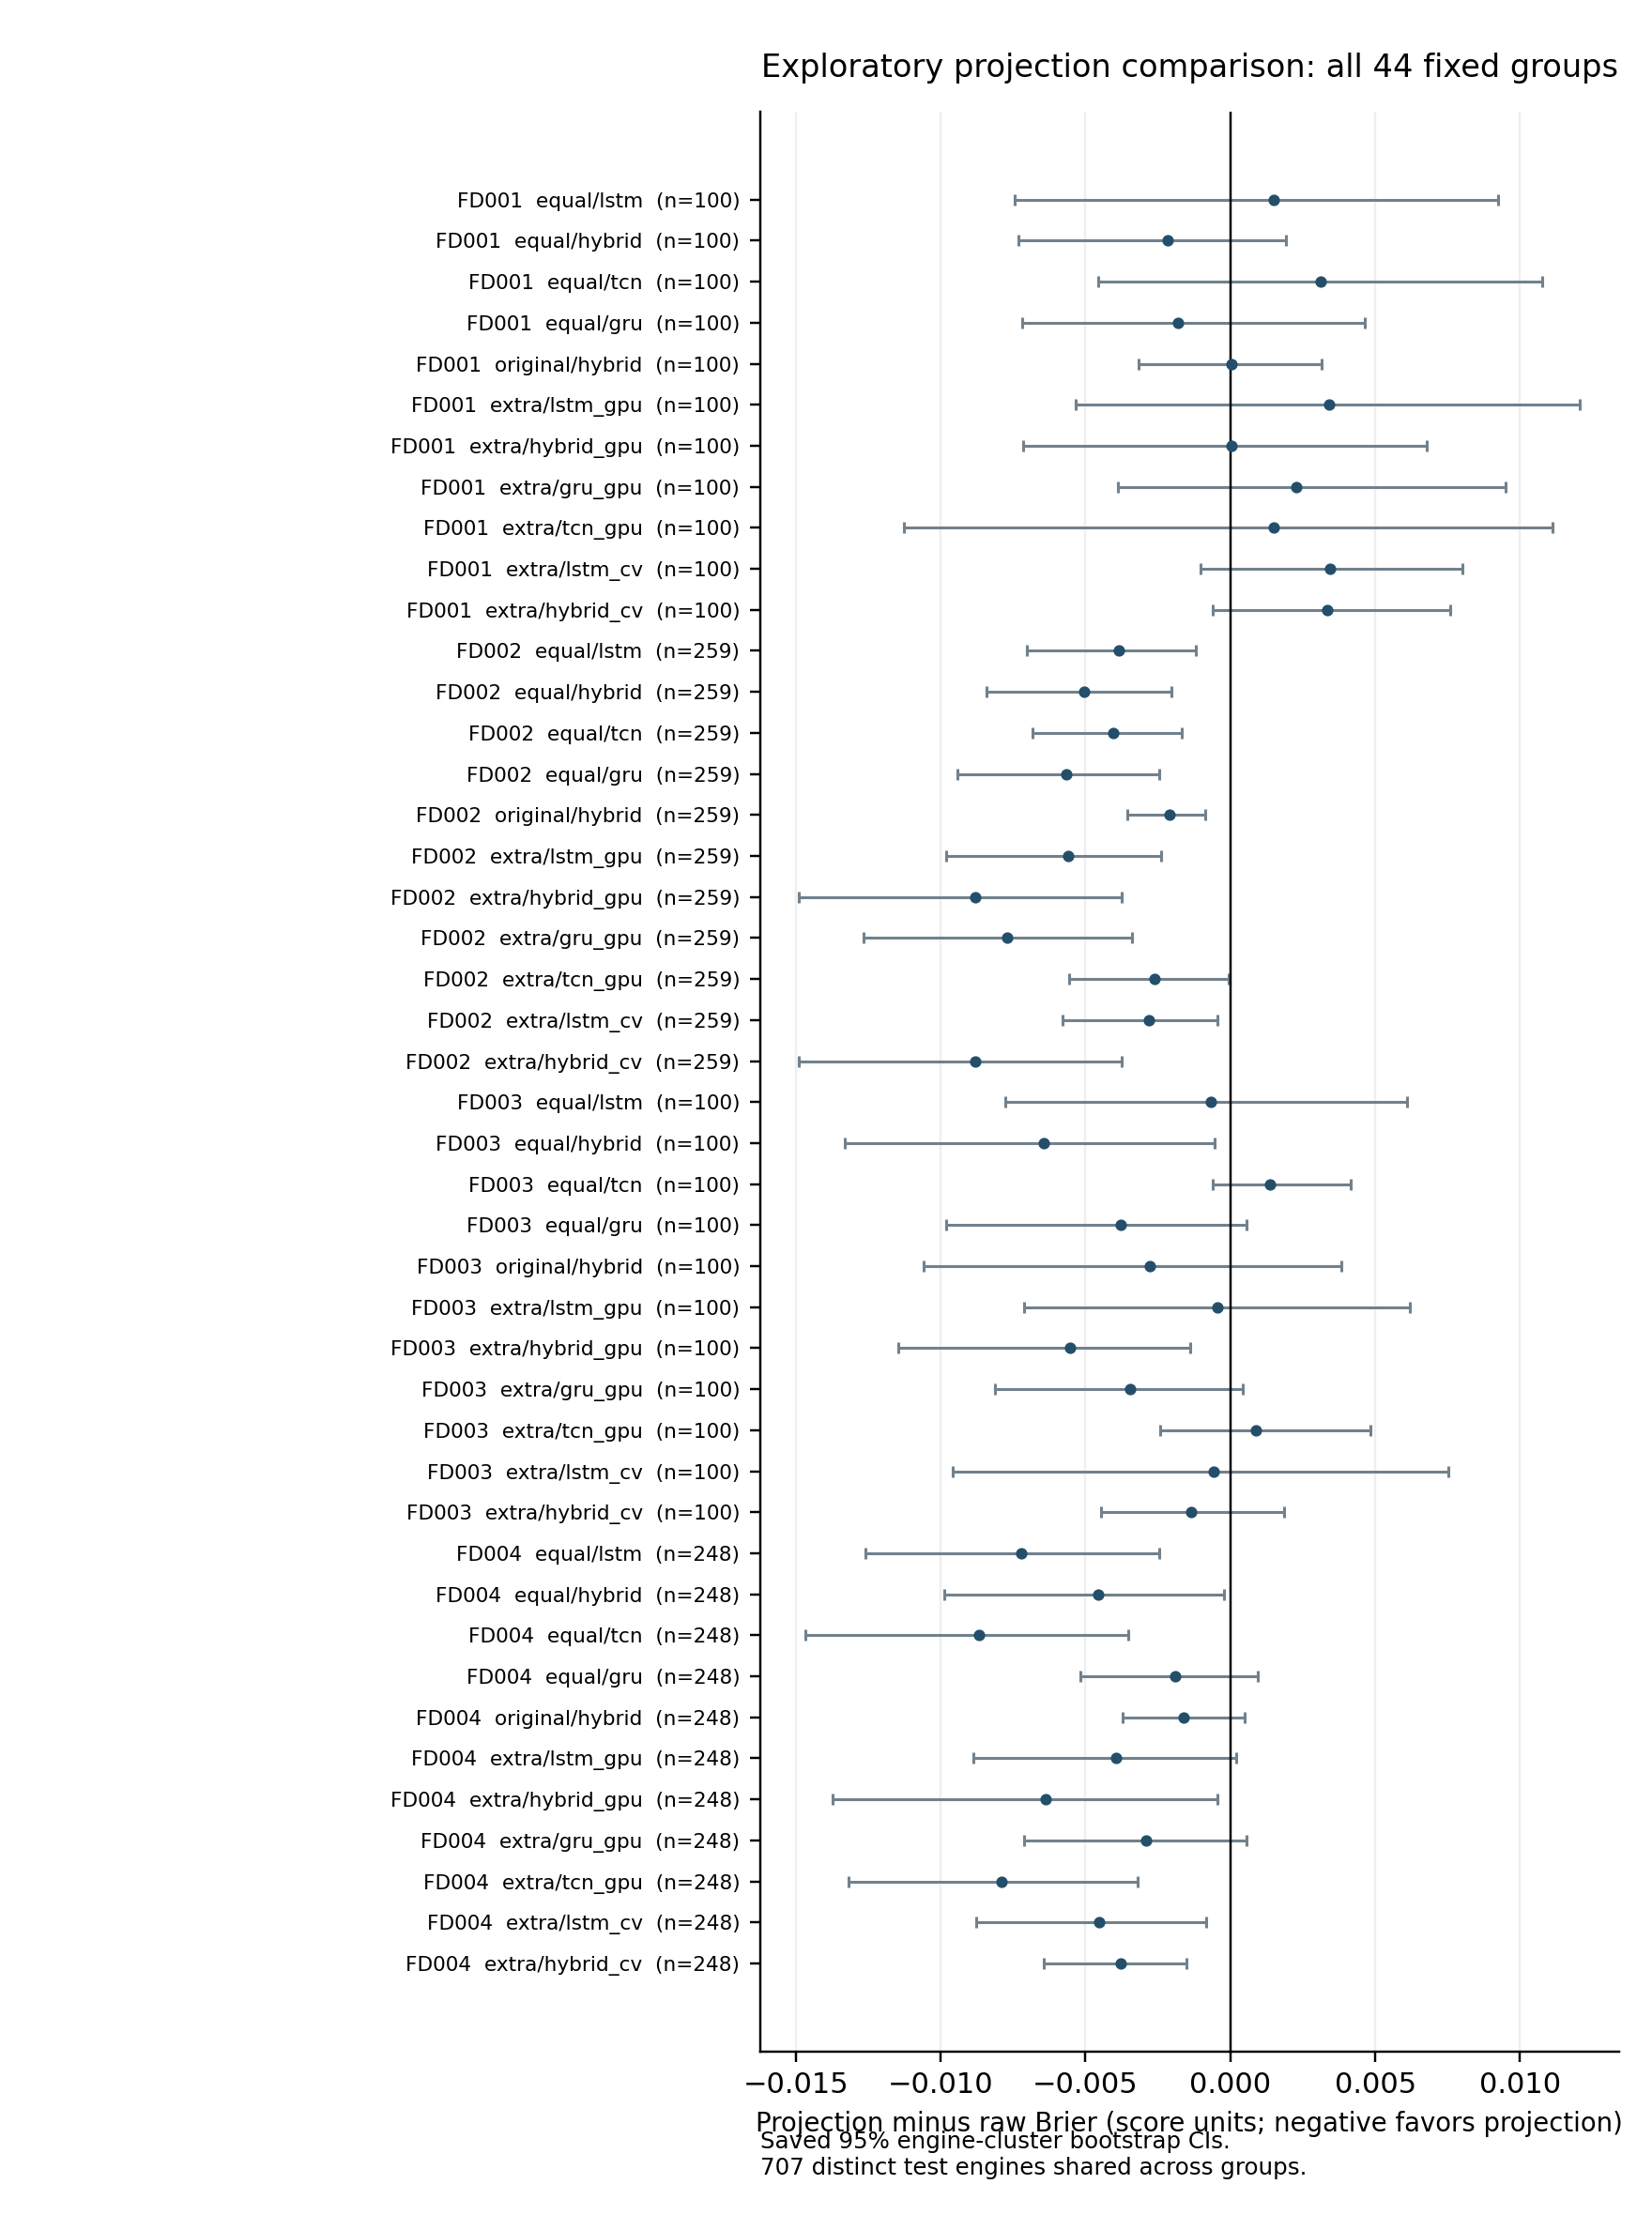
\includegraphics[width=\textwidth,height=0.81\textheight,keepaspectratio]{projection_brier_44_groups.png}
\caption{Projection-minus-raw Brier across the expanded 44-group roster. Points and 95\% engine-bootstrap CIs are copied from A\_\allowbreak{}all\_\allowbreak{}scores.csv; lower values favor projection. Labels show test engines per group: FD001 100, FD002 259, FD003 100 and FD004 248. All 44 groups share 707 distinct official-test engines; fixed fits do not multiply these counts.}
\end{figure*}

For practitioners, these results support reporting compatibility alongside proper scores. Projection can enforce the quantile-implied bounds without calibration labels, but should not be selected on an assumption of uniform scoring improvement. Training-weight correction addresses a different source of probability displacement and should likewise be assessed for the relevant subset and outcome. The present comparisons do not establish a benefit for maintenance decisions or operational safety.

\section{Limitations and conclusion}

The diagnostic detects the tested gross event-head corruptions, with sensitivity that depends on corruption direction. Its threshold concentration and adjusted associations do not establish general fault detection, and the negative median-error associations remain unexplained. This is an exploratory study using examined data from a single benchmark. The expanded \mbox{44} groups share the same \mbox{707} engines, so additional model configurations do not supply independent-engine replication. Bootstrap CIs condition on the fitted models, calibration maps and analysis choices. DS01 (\mbox{4} test engines) was descriptive only and was not validated \cite{ariaschao2021ncmapss}.

Projection supplies a label-free guarantee of the necessary structural bounds, with a small and inconsistent scoring gain. TrainOff has lower pooled Brier and NLL than projection alone, largely driven by FD002, while individual groups can favor projection. Neither compatibility alone nor a favorable pooled proper score establishes that a correction is suitable for every deployment. PHM evaluations should retain the distinction between structural agreement, probability error and point error, and report the adverse group results alongside pooled improvements.

\section*{Data and code availability}

The repository \url{https://github.com/amirhossein2004-mozafari/rul-quantile-event-compatibility} contains code, protocols, result CSVs, saved predictions, reports, manuscript sources and the supplement. It excludes \mbox{185} hash-referenced files, including checkpoints, tensors, raw NASA data and other inputs, so the public release cannot support full retraining or full lock verification. NASA data can be downloaded from the NASA Prognostics Center of Excellence repository (\url{https://www.nasa.gov/intelligent-systems-division/discovery-and-systems-health/pcoe/pcoe-data-set-repository/}). Code is licensed under MIT, and derived results and saved predictions are licensed under CC BY 4.0. The validation supplement contains Tables S1--S14 with source-file labels and full-precision companion tables. The repository also includes the added-model comparisons. Monitoring, PCGrad, component ablations, path-maximum CV+ and multi-study comparisons remain supplementary.

\section*{Authorship, funding and competing interests}

Amirhossein Mozafari: conceptualization, methodology, software, validation, analysis, investigation, data curation, writing, visualization and project administration. No specific external funding was received. The author declares no known competing financial interests or personal relationships affecting this work.

\section*{Declaration of generative AI assistance}

Generative AI tools assisted with code scripting and correction, analysis scripts, figure preparation and formatting, language editing, manuscript revision, and numerical checks. The author has manually reviewed, verified, and takes full responsibility for all methodology, code, numerical results, and manuscript content.

\clearpage
\bibliographystyle{apacite}
\PHMbibliography{references}
\end{document}
